\begin{block}{Hardware}

\begin{multicols}{2}
\begin{itemize}
\footnotesize
    \item To accelerate Memcached lookups, we add two additional hardware
        blocks, the traffic manager and the accelerator.
    \item The accelerator takes in a key and computes primary and secondary
        hash values, which it uses to look up the value stored in its local
        block RAM.

    \item The traffic manager sits between the NIC and the DMA engine and
        intercepts Memcached Get requests. It then queries the accelerator
        and sends the reply back to the NIC if the key is found.
\end{itemize}

\columnbreak
\begin{center}
    \includegraphics[width=\linewidth]{img/kvstore.pdf}
\end{center}
\hrule
\begin{center}
    \includegraphics[width=\linewidth]{img/frontend.pdf}
\end{center}

\end{multicols}

\end{block}
